Before continuing to the visualization part, it is worth to define the blockchain system that we refer to. Because the research of blockchain technology is still in progress, there are different methods and approaches used to construct a blockchain system. In this chapter, we introduce the ideas of the blockchain system that serves as the basis of the visualization.

\section{Data Types}

There are only two types of data structures that are used in the blockchain system: \textit{transactions} and \textit{blocks}. They are published and received by nodes continuously in the same blockchain network. A transaction contains information that is used in the blockchain system, such as a trade of cryptocurrecy or a shopping item. A block contains a number of transactions that are mined by a miner, and blocks are chained together to form a tree structure that represents the blockchain data structure. The transactions that are included in a block are considered to be confirmed if the block is at the longest blockchain.

\begin{table}[htb]
    \centering
    \begin{tabular}{ M{2cm}|m{8cm} } 
        \hline
        \multicolumn{2}{c}{\textbf{Transaction}} \\
        \hline
        \textit{Properties} & \multicolumn{1}{c}{\textit{Description}} \\
        \hline
        ID & the hash value of the transaction. \\ 
        type & is always “transaction”. \\ 
        timestamp & the time that the transaction is created. \\ 
        reward & the number of rewards that the miner will receive. \\ 
        privilege & to prevent the starvation of the transaction. \\ 
        \hline
    \end{tabular}
    \caption{Properties of Transactions.}
    \label{tab:properties of transactions}
\end{table}

For transactions (Table \ref{tab:properties of transactions}), the properties contain the ID, the type, the timestamp, the reward, and the privilege. The ID represents the hash value of the transaction in a blockchain system. Here we use 8 random characters and digits to simplify the representation. The type indicates that the data is a valid transaction data structure. The timestamp is decided at the time the transaction is created. 

The reward and the privilege are related to the mining strategies. The \textit{value} of a transaction is the sum of the reward and the privilege, as the equation \ref{eq:transaction value} states.

\begin{equation} \label{eq:transaction value}
    value = reward + privilege
\end{equation}

Miners can set the minimum value of transactions that are qualified to be mined. The reward is the number of money that will be assigned to the miner as a motivation because miners solve puzzles in a proof-of-work based blockchain system. The privilege is set to 0 when a transaction is created, and it is added by a sepcific number if the transaction is not selected to be mined each time during the mining activities. That is, the privilege prevents the transaction from starvation, i.e., the transaction will not have chance to be mined because of its low reward.

To explain the value of transactions clearly, suppose that a transaction with reward of 5 was generated and published, and a miner, Alice, received this transaction. At this time, Alice set the privilege of this transaction to 0. Now the total value of this transaction is 

\begin{gather*}
    reward = 5 \\
    privilege = 0 \\
    value = reward + privilege = 5 + 0 = 5
\end{gather*}

Assume that Alice decides to mine a block, but she does not select this transaction as one of the candidates because Alice expects that the minimum value of transactions should be 6. Therefore, the privilege of this transaction is added by a sepcific number (1 in this example). Now the value of this transaction is

\begin{gather*}
    reward = 5 \\
    privilege = 1 \\
    value = reward + privilege = 5 + 1 = 6
\end{gather*}

Thus, when Alice decides to mine a block next time, she will select this transaction as one of the candidates because the value of this transaction is not less than 6. It demonstrates that the privilege prevents this transaction from starvation. Actually, we design this mechanism because a transaction should not be ignored forever in a real blockchain system such as Bitcoin, even if the reward of the transaction is very low.

\begin{table}[htb]
    \centering
    \begin{tabular}{ M{2cm}|m{8cm} } 
        \hline
        \multicolumn{2}{c}{\textbf{Block}} \\
        \hline
        \textit{Properties} & \multicolumn{1}{c}{\textit{Description}} \\
        \hline
        ID & the hash value of the block. \\ 
        type & is always “block”. \\ 
        timestamp & the time that the block is created. \\ 
        miner & the public address of the miner. \\ 
        previous & the hash value of the previous block. \\ 
        layer & indicates the position of the block in the blockchain. \\ 
        color & the color of the block. \\ 
        transactions & an array of transactions. \\ 
        \hline
    \end{tabular}
    \caption{Properties of Blocks.}
    \label{tab:properties of blocks}
\end{table}

For blocks (Table \ref{tab:properties of blocks}), the properties contain the ID, the type, the timestamp, the miner, the previous, the layer, the color, and the transactions. The ID represents the hash value of the block in a blockchain system. Here we use also 8 random characters and digits as the hash value. The type indicates that the data is a valid block data structure. The timestamp is decided at the time the block is created. The miner represents the public address of the miner who mined this block, and it is a 8 random characters and digits. The previous contains the ID of the previous block that is chained in the same blockchain. The transactions includes an array of transactions, and the total reward of the block is the sum of these transactions.

The layer and color are useful for the visualization of the blockchains. The layer defines the position of a block in a blockchain and ensures that the visualization of the structures of blockchains between different nodes is the same. The color distinguishes the miner of the blocks in the visualization. The blocks with the same color mean that these blocks are from the same miner and vice versa.

\begin{figure}[htb]
    \centering
    \begin{subfigure}[b]{0.4\textwidth}
        \centering
        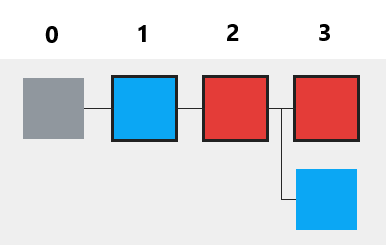
\includegraphics[width=\textwidth]{blockchain_block1}
        \caption{Alice's blockchain}
    \end{subfigure}
    \hfill
    \begin{subfigure}[b]{0.4\textwidth}
        \centering
        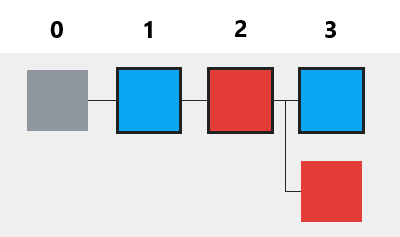
\includegraphics[width=\textwidth]{blockchain_block2}
        \caption{Bob's blockchain}
    \end{subfigure}

    \caption{Visualization of Blocks.}
    \label{fig:visualization of blocks}
\end{figure}

To illustrate the positions of blocks in the visualization, suppose that there are two miners, Alice and Bob. Alice's color is red, and Bob's color is blue. According to figure \ref{fig:visualization of blocks}, Alice and Bob mined two block individually. The grey block represents the genesis block. The red blocks are from Alice, and the blue ones are from Bob. The number of layers of the blocks are indicated on the top of the figures. In each layer, the number of different color of blocks are the same. However, the vertical positions of the blocks are not always the same. It is because that each miner received the same block at different time. In this example, Alice and Bob put their own blocks on the top of the layer because they received their own blocks earlier. As a result, the layer guarantees that the blockchain data structures are the same between every node.

\section{Nodes}

In the blockchain system, there are three types of nodes that communicate with each other. 
\begin{itemize}
    \item \textbf{Transaction Generator} \\
        The transaction generator is unique in the blockchain system. It is responsible for generating and publishing transactions to miners.
    \item \textbf{Miner} \\
        Miners are the most important nodes in the visualization because they mine and publish blocks according to their individual mining strategies. Each miner has their own transaction pools which contain all the pending transactions. Because the transaction generator publishes the transactions through the unstable network, each miner has different sets of pending transactions at the same time.
    \item \textbf{Nonminer} \\
        Nonminers only receive blocks from miners and publishes blocks to their neighbors.
\end{itemize}

The blockchain data structures of different nodes are not always the same since the blockchain system is active. It is because of the delays of the unstable network between different nodes, and the visualization of the different blockchain data structures is the main feature of our application. For example, figure \ref{fig:visualization of blocks} shows the difference between Alice's and Bob's blockchain data structures.

\begin{figure}[htb]
    \centering
    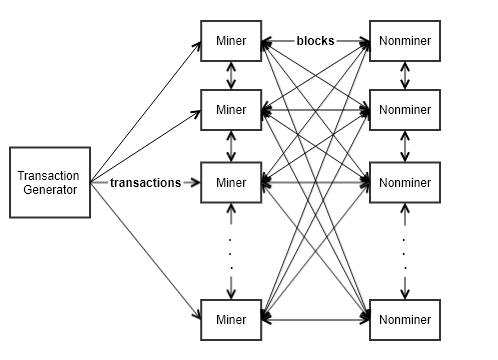
\includegraphics[width=\textwidth]{blockchain_nodes}
    \caption{Relationships of Nodes.}
    \label{fig:relationship of nodes}
\end{figure}

The relationship of different types of nodes is shown in figure \ref{fig:relationship of nodes}. In the beginning, the transaction generator publishes transactions to the miners. When a miner mines a block, he/she will publish the block through his/her neighbors. Other miners and nonminers will again publish the received block to their neighbors after they received the block from other miners or nonminers. If a miner or a nonminer receives duplicate blocks, then he/she will discards the block to prevent sending and receiving the same block repeatedly.

\section{Unstable Networks}

The networks between each node are unstable due to the characteristic of peer-to-peer networks. Therefore, the publishes of transactions and blocks suffer delays. Because of the unstable network, forks happen in the visualization of the blockchains while several miners are mining simultaneously. Moreover, nodes could be partitioned into different groups and compete with other groups.

\begin{figure}[htb]
    \centering
    \begin{subfigure}[b]{1\textwidth}
        \centering
        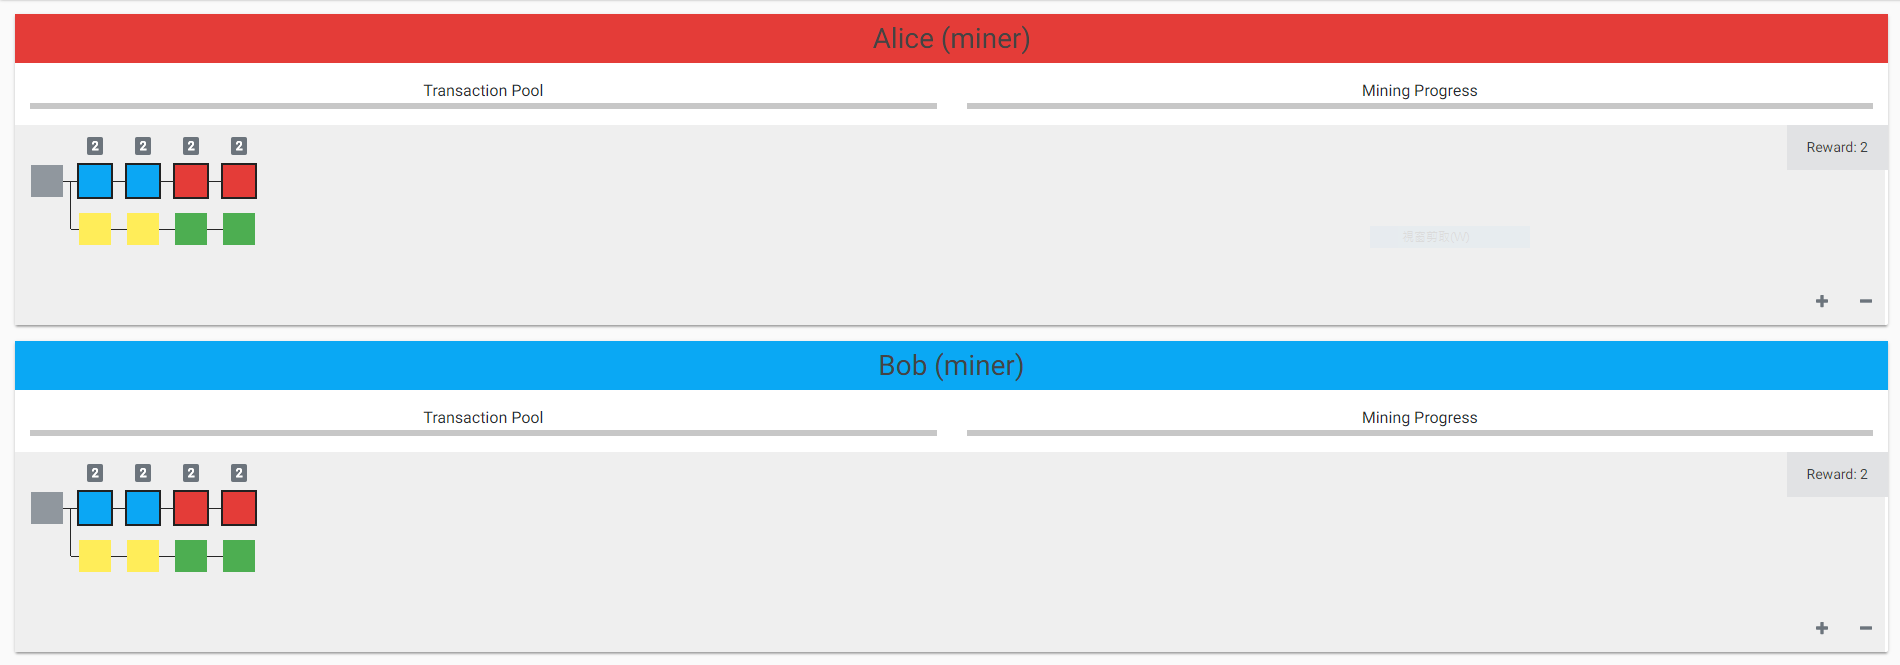
\includegraphics[width=\textwidth]{blockchain_delays1}
        \caption{Group 1}
    \end{subfigure}
    
    \begin{subfigure}[b]{1\textwidth}
        \centering
        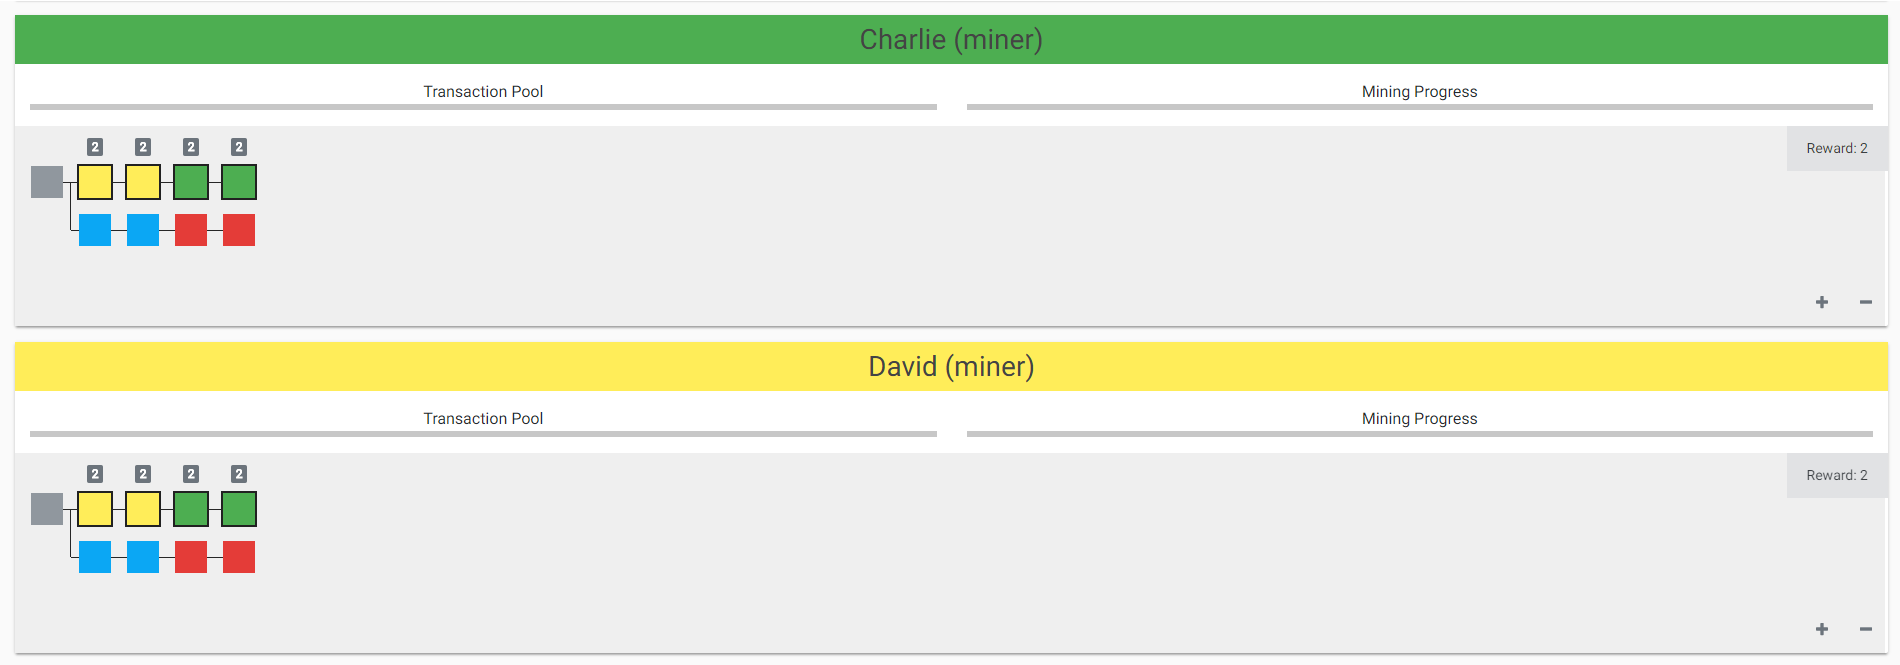
\includegraphics[width=\textwidth]{blockchain_delays2}
        \caption{Group 2}
    \end{subfigure}

    \caption{Groups of Miners.}
    \label{fig:groups of miners}
\end{figure}

For example, in figure \ref{fig:groups of miners}, there are two groups of miners, and they are partitioned because different groups suffer high delays between each other, and the networks of the miners in the same group are much faster. Therefore, the miners in the same group consider that their own blockchain is the longest.

\section{Mining Strategies}

Every miner has different mining strategies. There are four parameters that influence the mining strategies and mining activities. 

\begin{itemize}
    \item \textbf{Mining Time} \\
        A miner needs a period of time to mine a block by solving the puzzles. Thus, this parameter reflects the computing power of miners and the difficulty of puzzles.
    \item \textbf{Minimum Value of Transactions} \\
        This parameter is used to select a set of candidate transactions that are considered to be mined into a block. It is the threshold of the values of transactions which are qualified to be selected when the miner decides to mine a block.
    \item \textbf{Fixed Number of Transactions in Blocks} \\
        This parameter is the size of a block. The sizes of blocks are always the same for the same miner.
    \item \textbf{Minimum Number of Pending Transactions} \\
        Miners store pending transactions in the transaction pools. This parameter prevents that a miner responds too slowly in the blockchain system when the minimum value of transactions is set by a large number.
\end{itemize}

The four parameters make the mining behaviors of the miners different from each other. The influences of mining strategies to the blockchain system under specific environment can be identified clearly through the visualization. More details of how mining strategies is applied in the mining activities can be found in section \ref{algorithms}.

\section{Consensus Protocols}

The consensus protocol that is applied in the blockchain system is proof-of-work. Under proof-of-work protocol, miners solve mathematical puzzles with their computing power. By comparing the blockchain data structures between each node, the longest blockchain can be identified easily. Miners always switch to the longest blockchain as soon as possible to ensure that they are working on the correct fork of blockchains. Additionally, miners only get rewards by adding blocks to the correct blockchain.

The parameters of the mining strategies are designed for proof-of-work protocol. Therefore, the parameters will be entirely different if the applied consensus protocol is changed, e.g., proof-of-stake, in the future.